\subsection{Kennzahlen}
    Auch in diesem Fallbeispiel wurde eine Reihe an Kennzahlen ermittelt,
    die in diesem Kapitel präsentiert werden.

    \paragraph{Struktur eines Graphs}
    Zum Verständnis der Zahlen trägt Abbildung \ref{image:findingNewsFiguresDbModel} bei,
    welches den Aufbau des Graphs visualisiert.
    Wegen der beschriebenen Überschneidung mit dem ersten Fallbeispiel,
    sind die entsprechenden Knoten hier nicht nochmals dargestellt.
    Wie im vorherigen Beispiel wird außerdem auf die Darstellung von
    Referenzen verzichtet.

    \begin{figure}[htb]
        \centering
        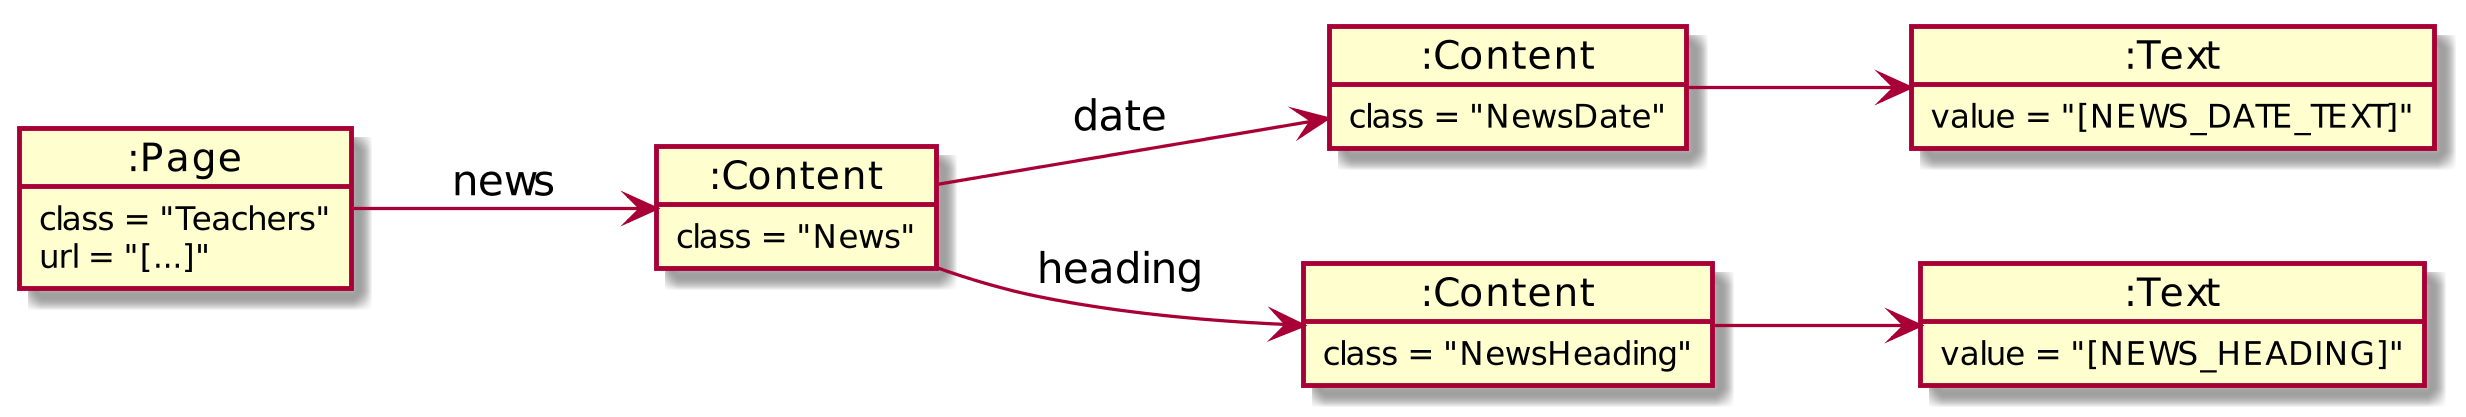
\includegraphics[scale=\imageScalingFactor]{../resources/findings/case-study-2/dbmodel.png}
        \caption{Struktur des Graphs einer Seite über aktuelle Meldungen}
        \label{image:findingNewsFiguresDbModel}
    \end{figure}

    \paragraph{Präsentation der Kennzahlen}
    Die folgenden Tabellen präsentieren die gesammelten Kennzahlen.
    Die Bedeutung einzelner Kennzahlen wurde bereits beim ersten Beispiel erläutert,
    die entsprechend auch hier gelten.
    Die Gruppierung der Knoten nach ihren Labels ist in Tabelle
    \ref{table:findingsNewsFiguresNodesByLabel} zu sehen.
    Die Häufigkeit der Inhaltsklassen stellt Tabelle
    \ref{table:findingsNewsFiguresContentNodesByClass} dar.
    Tabelle \ref{table:findingNewsFiguresEdgesByLabel} gruppiert die Kanten der Datenbank
    nach ihren Labels und Tabelle
    \ref{table:findingsNewsFiguresEdgesByStartEndNodeLabel}
    stellt heraus, welche Knotenarten diese Kanten verbinden.
    Zuletzt betrachtet Tabelle \ref{table:findingsNewsFiguresSharedNodes}
    die Frage, welche Knoten mehrfach referenziert wurden.

    \begin{table}[htb]
        \begin{subtable}[c]{0.3\textwidth}
            \centering
            \begin{tabular}{|l|c|}
                \hline
                \textbf{Label}  & \multicolumn{1}{l|}{\textbf{Anzahl}} \\ \hline
                Content         & 124                                  \\ \hline
                Page + Resource & 5                                    \\ \hline
                Resource        & 53                                   \\ \hline
                Site            & 1                                    \\ \hline
                Text            & 77                                   \\ \hline
                \hline
                \textbf{Summe}  & 260                                  \\ \hline
            \end{tabular}
            \subcaption{Knoten gruppiert nach Labels für Seiten über aktuelle Meldungen}
            \label{table:findingsNewsFiguresNodesByLabel}
        \end{subtable}
        \begin{subtable}[c]{0.3\textwidth}
            \centering
            \begin{tabular}{|l|c|}
                \hline
                \textbf{Klasse} & \multicolumn{1}{l|}{\textbf{Anzahl}} \\ \hline
                Brand           & 1                                    \\ \hline
                Header          & 1                                    \\ \hline
                News            & 41                                   \\ \hline
                NewsDate        & 38                                   \\ \hline
                NewsHeading     & 41                                   \\ \hline
                PageHeading     & 1                                    \\ \hline
                Portal          & 1                                    \\ \hline
                \hline
                \textbf{Summe}  & 260                                  \\ \hline
            \end{tabular}
            \subcaption{\texttt{Content}-Knoten gruppiert nach ihrer Klasse für Seiten über aktuelle Meldungen}
            \label{table:findingsNewsFiguresContentNodesByClass}
        \end{subtable}
        \begin{subtable}[c]{0.3\textwidth}
            \centering
            \begin{tabular}{|l|c|}
                \hline
                \textbf{Label} & \multicolumn{1}{l|}{\textbf{Anzahl}} \\ \hline
                Reads          & 80                                   \\ \hline
                References     & 87                                   \\ \hline
                Owns           & 145                                  \\ \hline
                \hline
                \textbf{Summe} & 312                                  \\ \hline
                \end{tabular}
            \subcaption{Kanten gruppiert nach Labels für Seiten über aktuelle Meldungen}
            \label{table:findingNewsFiguresEdgesByLabel}
        \end{subtable}

        \begin{subtable}[c]{0.5\textwidth}
            \centering
            \begin{tabular}{|l|c|}
                \hline
                \textbf{Start $\rightarrow$ Ziel} & \multicolumn{1}{l|}{\textbf{Anzahl}} \\ \hline
                (:Content) $\rightarrow$ (:Content)     & 83                                   \\ \hline
                (:Content) $\rightarrow$ (:Resource)    & 49                                   \\ \hline
                (:Page) $\rightarrow$ (:Content)        & 57                                   \\ \hline
                (:Page) $\rightarrow$ (:Page)           & 13                                   \\ \hline
                (:Page) $\rightarrow$ (:Resource)       & 25                                   \\ \hline
                (:Site) $\rightarrow$ (:Page)           & 5                                    \\ \hline
                \textbf{Summe}                    & 232                                  \\ \hline
            \end{tabular}
            \subcaption{Kanten gruppiert nach Labels der Start- und Zielknoten für Seiten über aktuelle Meldungen}
            \label{table:findingsNewsFiguresEdgesByStartEndNodeLabel}
        \end{subtable}
        \begin{subtable}[c]{0.5\textwidth}
            \centering
            \begin{tabular}{|l|c|}
                \hline
                \textbf{Knoten} & \multicolumn{1}{l|}{\textbf{Anzahl}} \\ \hline
                PageHeading     & 1                                    \\ \hline
                Portal          & 1                                    \\ \hline
                Header          & 1                                    \\ \hline
                News            & 1                                    \\ \hline
                NewsDate        & 1                                    \\ \hline
                Seiten          & 4                                    \\ \hline
                Unterseiten     & 5                                    \\ \hline
                :Text           & 2                                    \\ \hline
                \textbf{Summe}  & 16                                   \\ \hline
                \end{tabular}
            \subcaption{Knoten mit mehreren eingehenden Kanten für Seiten über aktuelle Meldungen}
            \label{table:findingsNewsFiguresSharedNodes}
        \end{subtable}
        \label{table:findingsNewsFigures}
        \caption{Kennzahlen der Seiten über aktuelle Meldungen}
    \end{table}